\subsection{Layer deduplication}
\label{sec:dedup-desgin}

%We now describe \sysname's layer restoring performance--aware deduplication 
% (i.e., \sysname's~\dedupname) system design. 

%\subsubsection{When to deduplicate layers?}
%

%
%Consider that deduplication incurs a performance overhead 
%and the current Docker registry already stores layers in compressed format to 
%save space and network transfer overhead. 
%We first analyze the space efficiency of a registry 
% that performs decompression and file-level deduplication and compare it to 
% a registry that naively stores compressed layers.
%
%In Figure~\ref{fig:cacheefficiency}, the x-axis values correspond to the sizes of $5$ random samples 
%drawn from the whole dataset (detailed in~\cref{sec:dataset-analysis}). %and the size of the dataset in terms of capacity and layer count.
%For a traditional registry, the compressed layer tarballs will be kept as is.
%While a registry with file-level deduplication will store \emph{deduplicated} layers (i.e., unique files). 
%The y-axis shows how much space a registry with file-level deduplication can save compared to naively storing compressed layer tarballs.
%For the first two samples of the dataset, with size less than $20$~GB, 
%there is no benefit to \emph{deduplicate} layers 
%because the deduplication ratio is very low.
%However, when the dataset size is $3$~TB, we can save $56\%$ more space.
%The space saved by applying decompression and file-level deduplication increases almost linearly with the size of the layer dataset.
%This verifies the benefit of deduplicate layers when the dataset is large, 
%which should be carefully selected to realize significant space savings.

%\subsubsection{Layer deduplication and partition}


Similar with traditional registry, 
\sysname maintains a \emph{layer index} to address the corresponding layers stored in the system.
After receiving a \texttt{push} layer request,
\sysname first checks the \textbf{layer fingerprint} in the \emph{layer index} to ensure 
an identical layer is not already stored.
Layer fingerprint is calculated by hashing the layer content, which is also used as layer identifier denoted as \textbf{layer id}.
After that, \sysname~stores the layer in stage area and acknowledges back to client. 
Meanwhile, \sysname will update \emph{RLmap} with the layer and its associated repository, where
RLmap maps a \textbf{repository id} (i.e., repository name) to its containing layers 
as shown in Figure~\ref{fig:dedup-partition}.
%After the layer is deduplicated, it will be removed from stage area.
%\dedupname system~initiates layer deduplication process only if 
%layer deduplication will achieve significant space savings and 
%the process won't impact foreground requests. 
%Sepcially, layer deduplication process is triggered when
%the layer dataset $S$ is greater than a predefined threshold $\theta_{s}$ and 
%the registry traffic $RPS$ ( i.e., requests per second) is lower than $\theta_{RPS}$. Thus, layer deduplication process runs periodically.
%The process always stars with the cold layers that haven't been
%access for a long time.
 
 \sysname initiates a lightweight layer deduplication process which collaborates with metadata database
 to remove the redundant files from layers. 
The deduplication process has three major steps: 
layer decompression and unpacking, 
file-level deduplication,
and \textbf{layer partition}. 
The first two steps are necessary for removing file duplicates from compressed layer tarballs.
The last step -- layer partition is to evenly distribute the I/O and computation load of layer restoring among multiple registry servers   
so that layer restoring process can achieve the maximum parallelism for each layer to
accelerate layer restoring process. 
%(detailed in~\cref{subsubsec:slice-restoring}) 
%After layer deduplication, unique files are evenly distributed across multiple registry servers. 
%We define all the per-server files belonging to a layer as a {\em slice}. 
%A server stores slices for many layers, and a layer is composed of slices stored on multiple servers, which allows restoring a layer in parallel. 
%\begin{figure*}[t]
%		\begin{minipage}{0.21\linewidth}
%			\centering
%			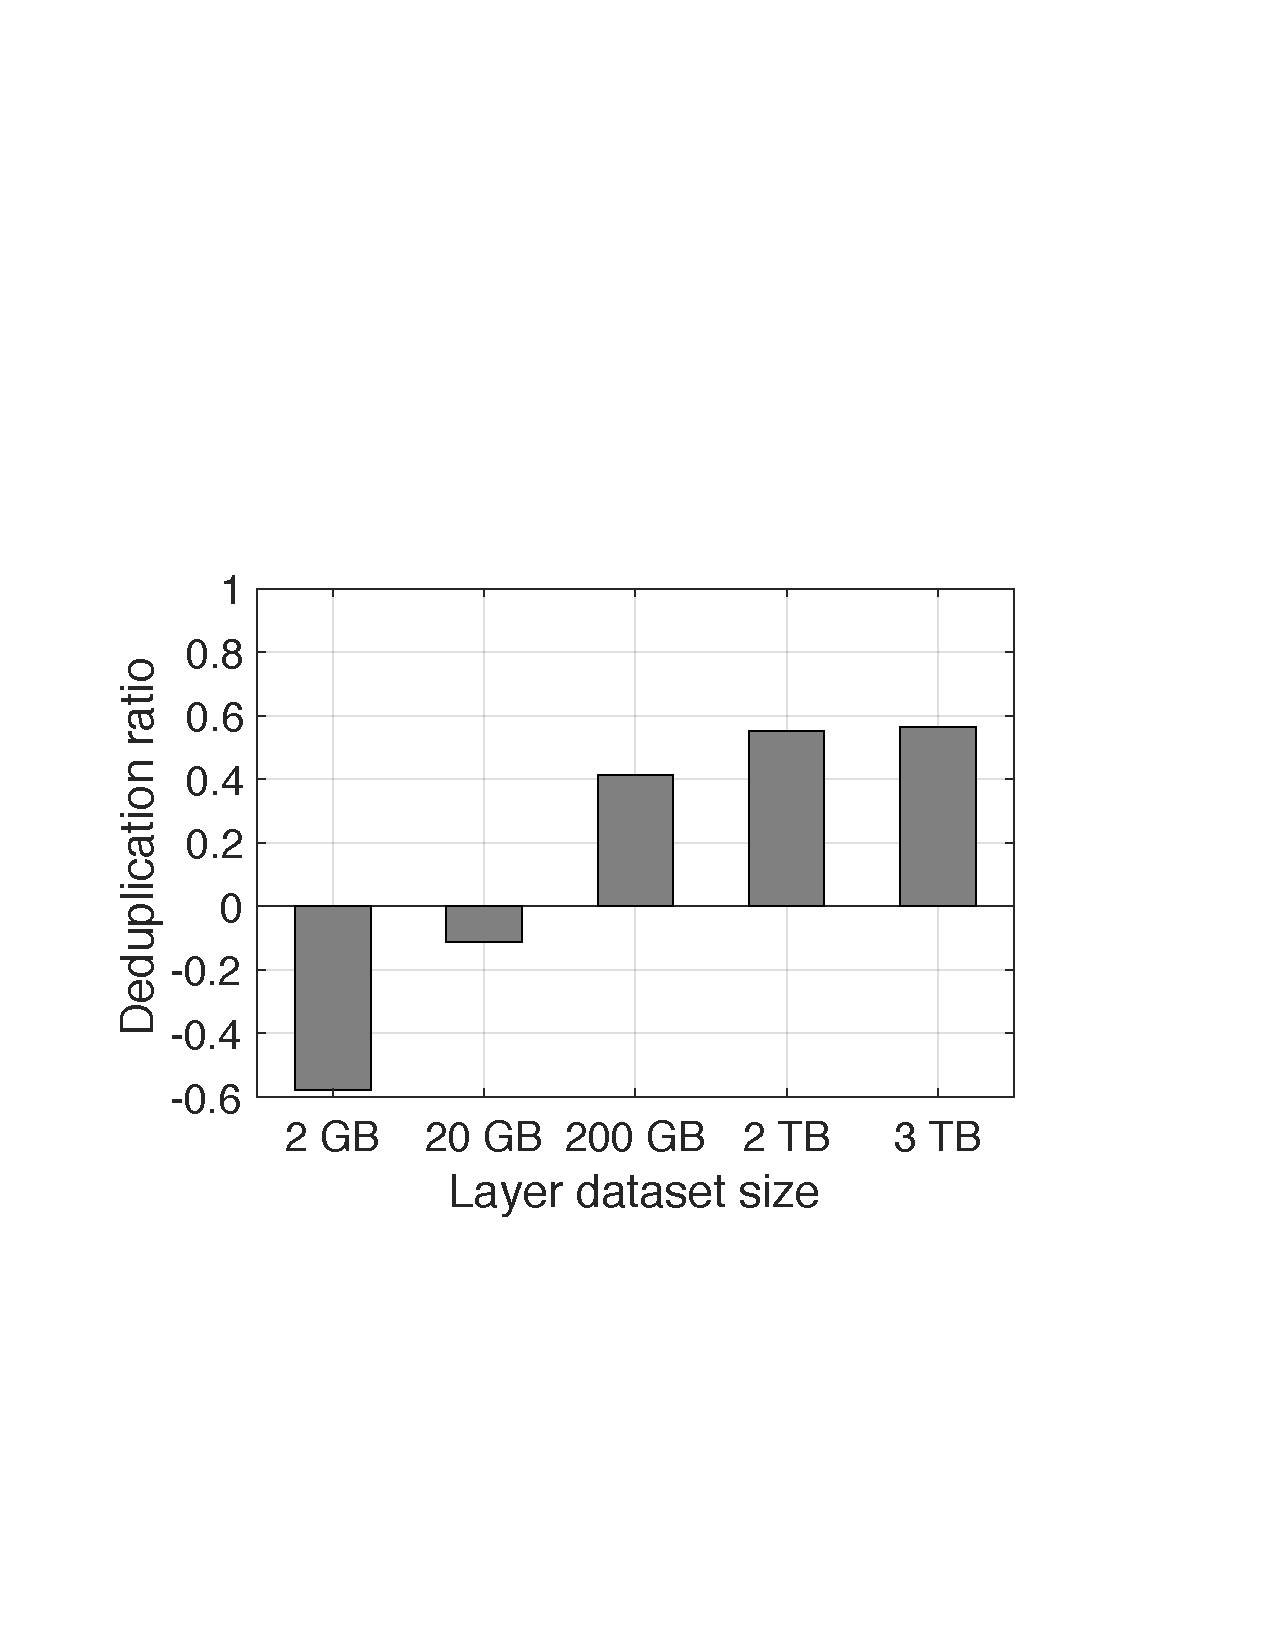
\includegraphics[width=1\textwidth]{graphs/dedup_vs_compression.pdf}
%			\caption{File-level deduplication vs. compression efficiency.}
%		%	\vspace{-3pt}
%			\label{fig:cacheefficiency}
%		\end{minipage}
%			\begin{minipage}{0.38\linewidth}
%				\centering
%				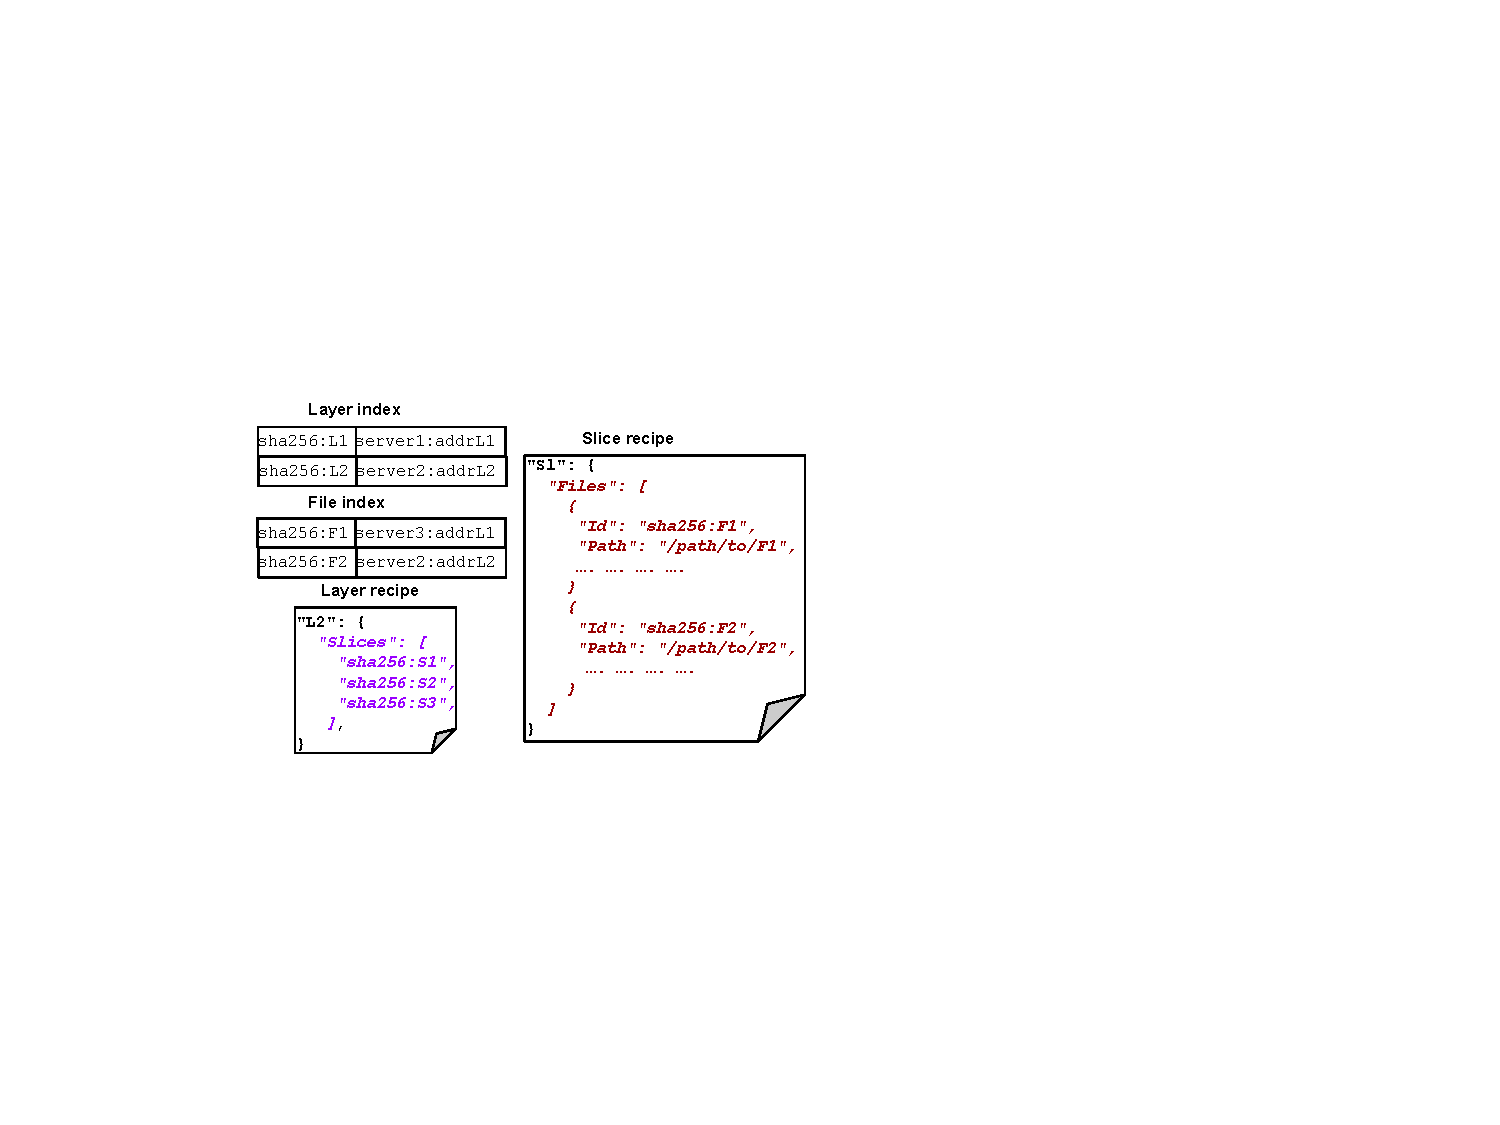
\includegraphics[width=1\textwidth]{graphs/sift-metadata.pdf}
%				\caption{Metadata for deduplication.}
%				%	\vspace{-3pt}
%				\label{fig:sift-metadata}
%			\end{minipage}
%		\begin{minipage}{0.38\linewidth}
%			\centering
%			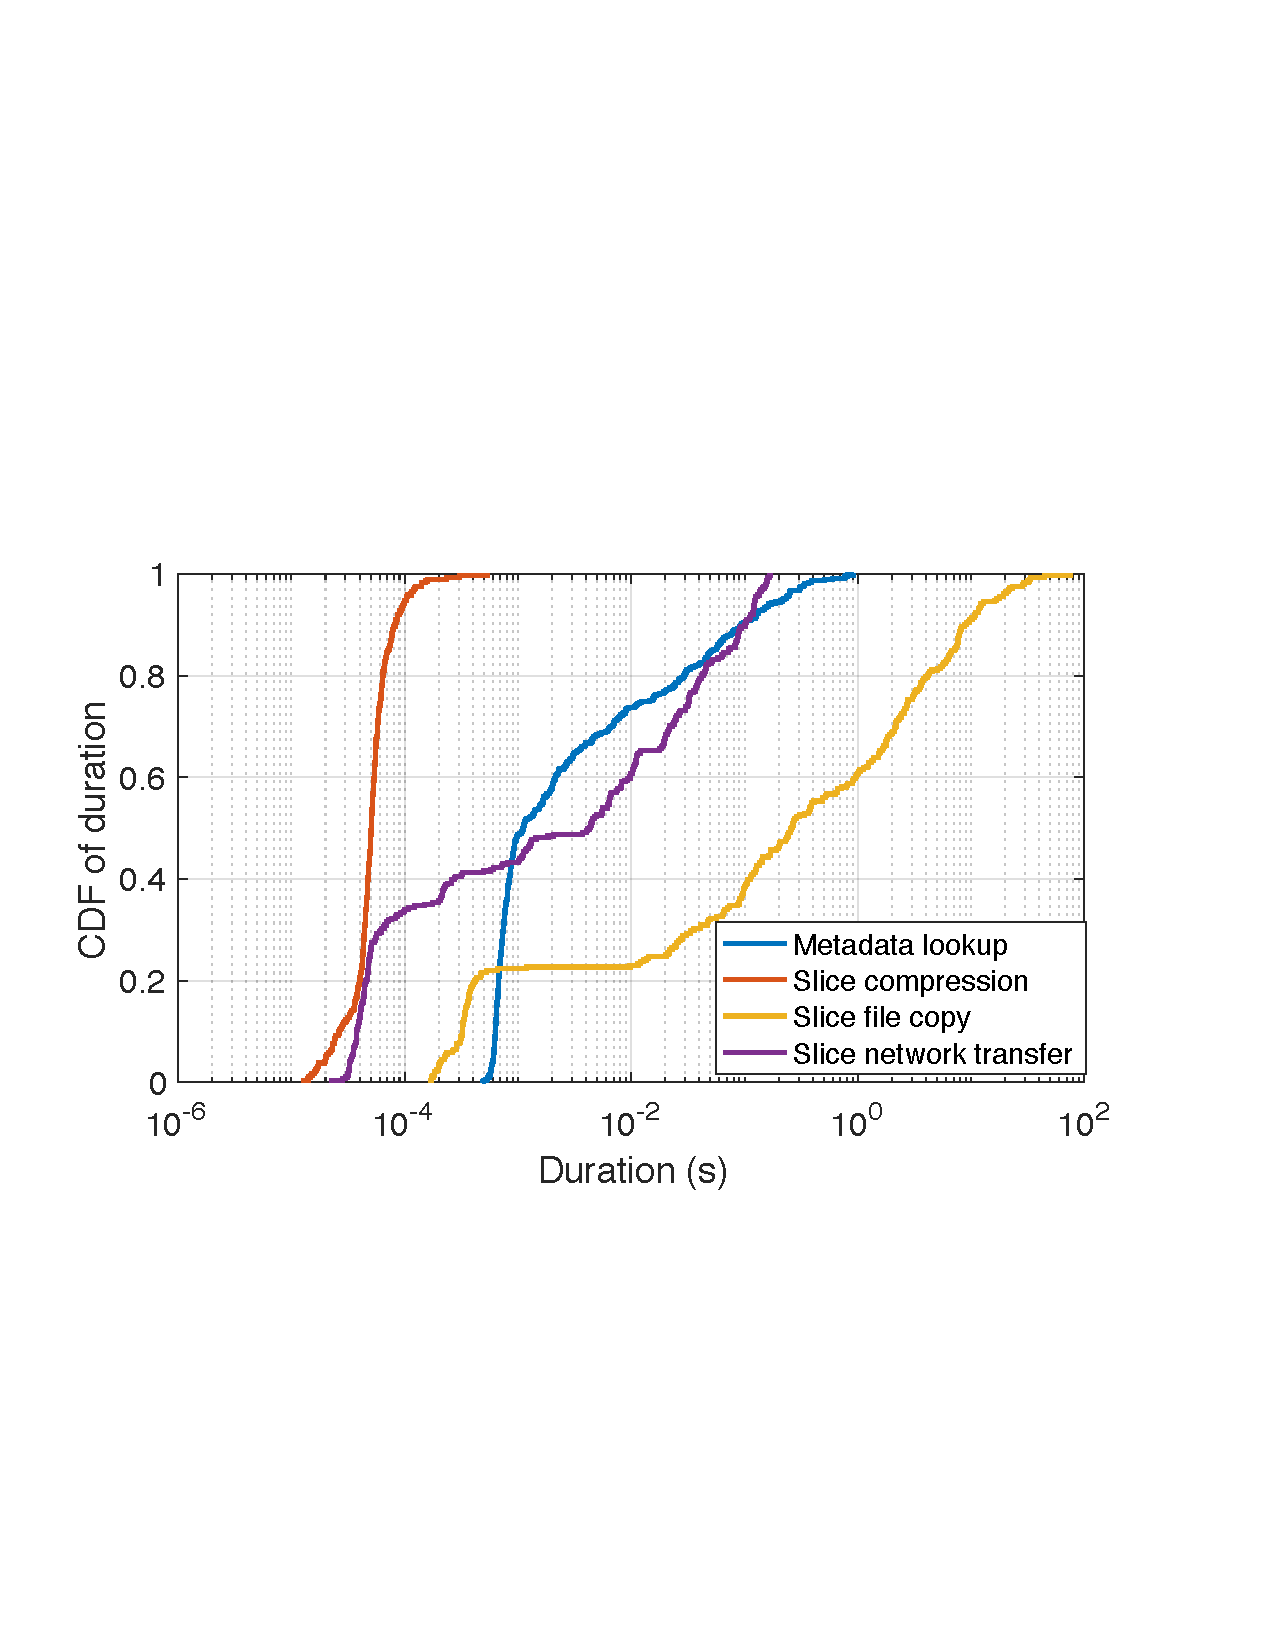
\includegraphics[width=1\textwidth]{graphs/restoring-breakdowns.pdf}
%			\caption{Breakdown of slice restoring time.}
%			%	\vspace{-3pt}
%			\label{fig:slice-restoring-breakdown}
%		\end{minipage}
%\end{figure*}

\begin{figure}[t]
	\centering
	\centering
	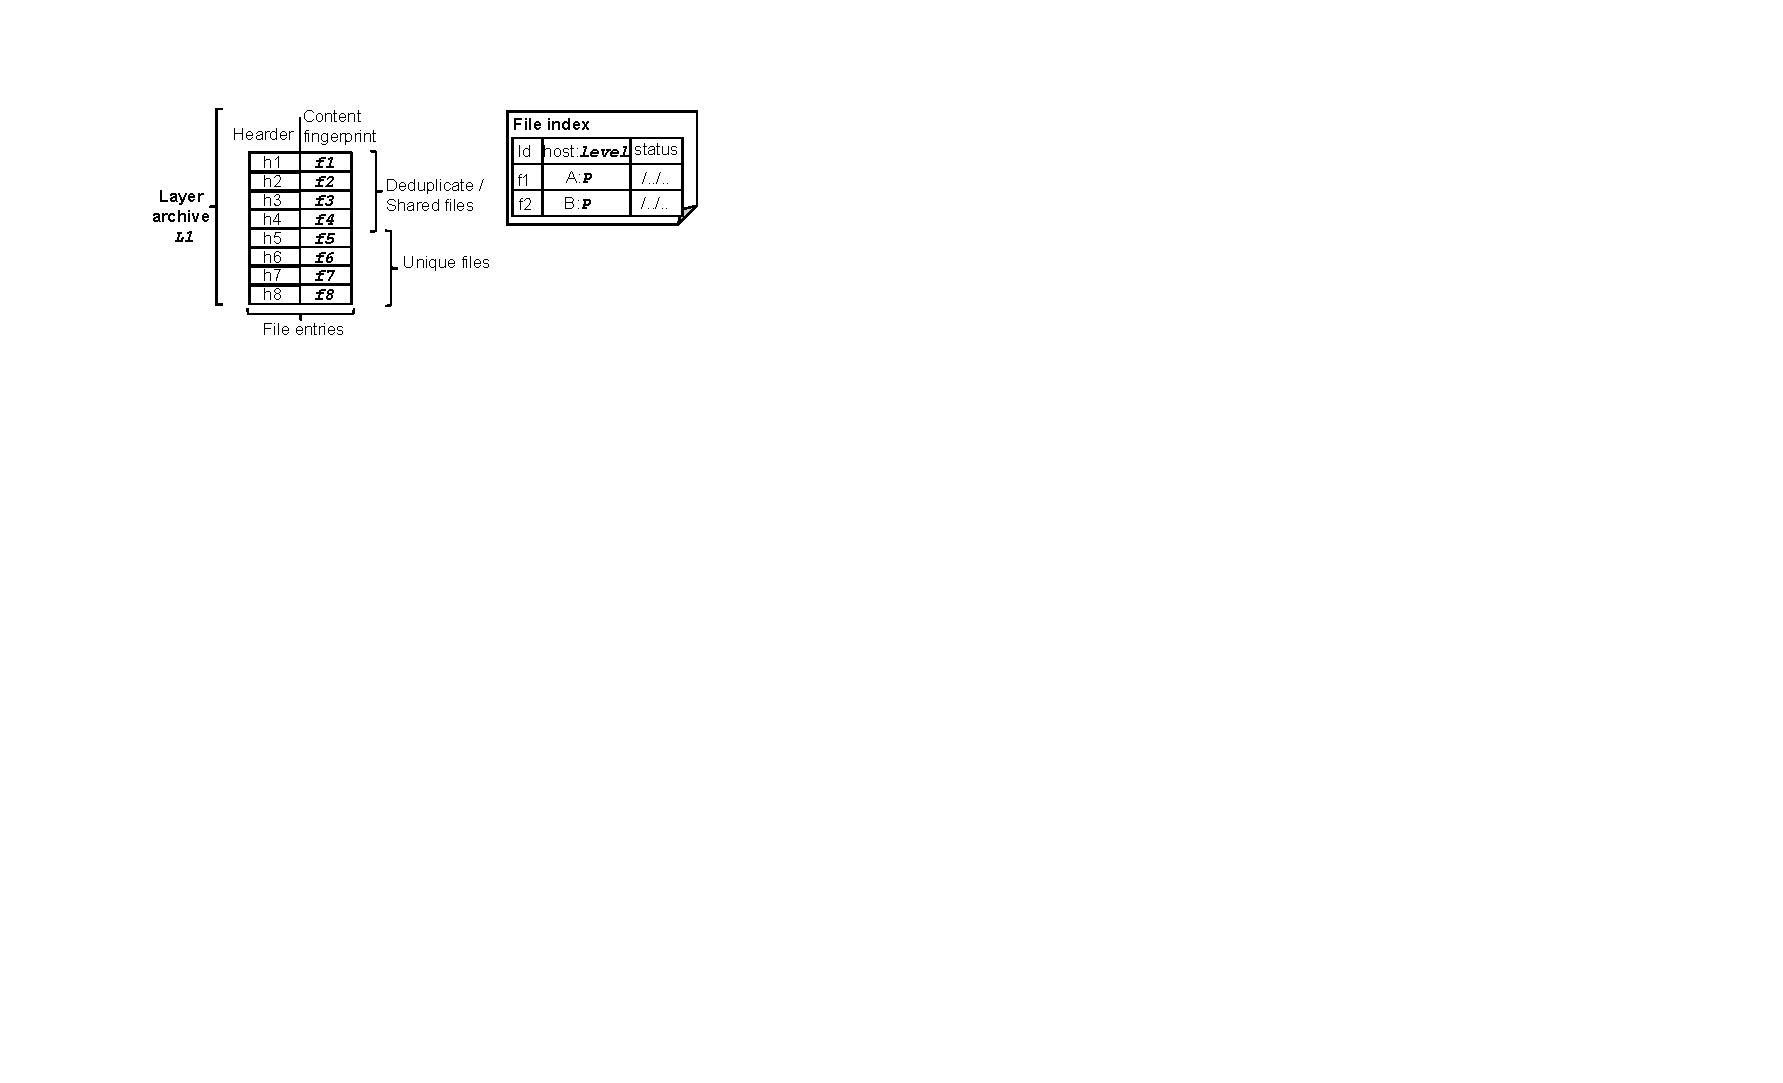
\includegraphics[width=0.45\textwidth]{graphs/sys-architecture-put-layer.pdf}
	\caption{Layer deduplication. \LR{Typo: ``Hearder'' should be ``Header''}}
	\label{fig:dedup-partition}
\end{figure}



%\begin{figure}[t]
%	\centering
%	\begin{minipage}{0.26\textwidth}
%		\centering
%		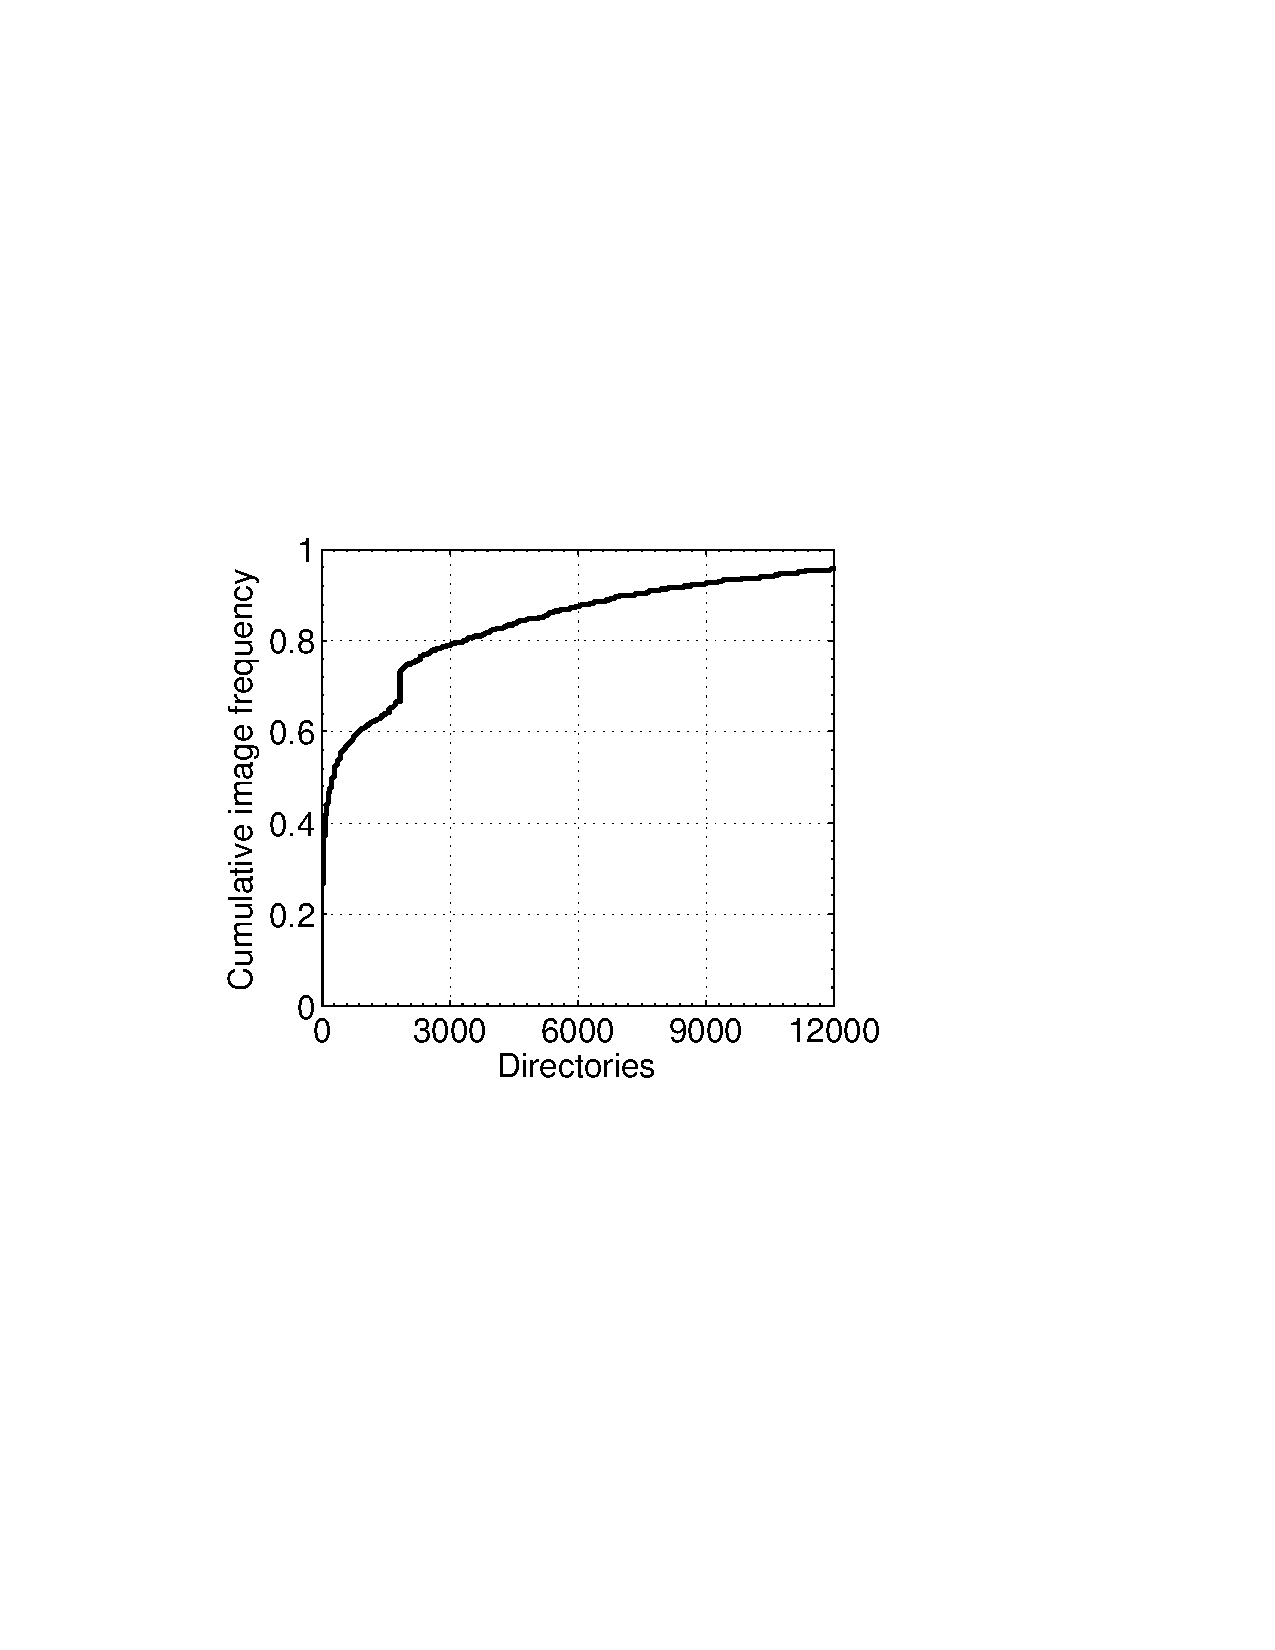
\includegraphics[width=1\textwidth]{graphs/dir.pdf}
%		\caption{CDF of images by\newline directories}
%		\label{fig-dir}
%	\end{minipage}%
%	\begin{minipage}{0.24\textwidth}
%		\centering
%		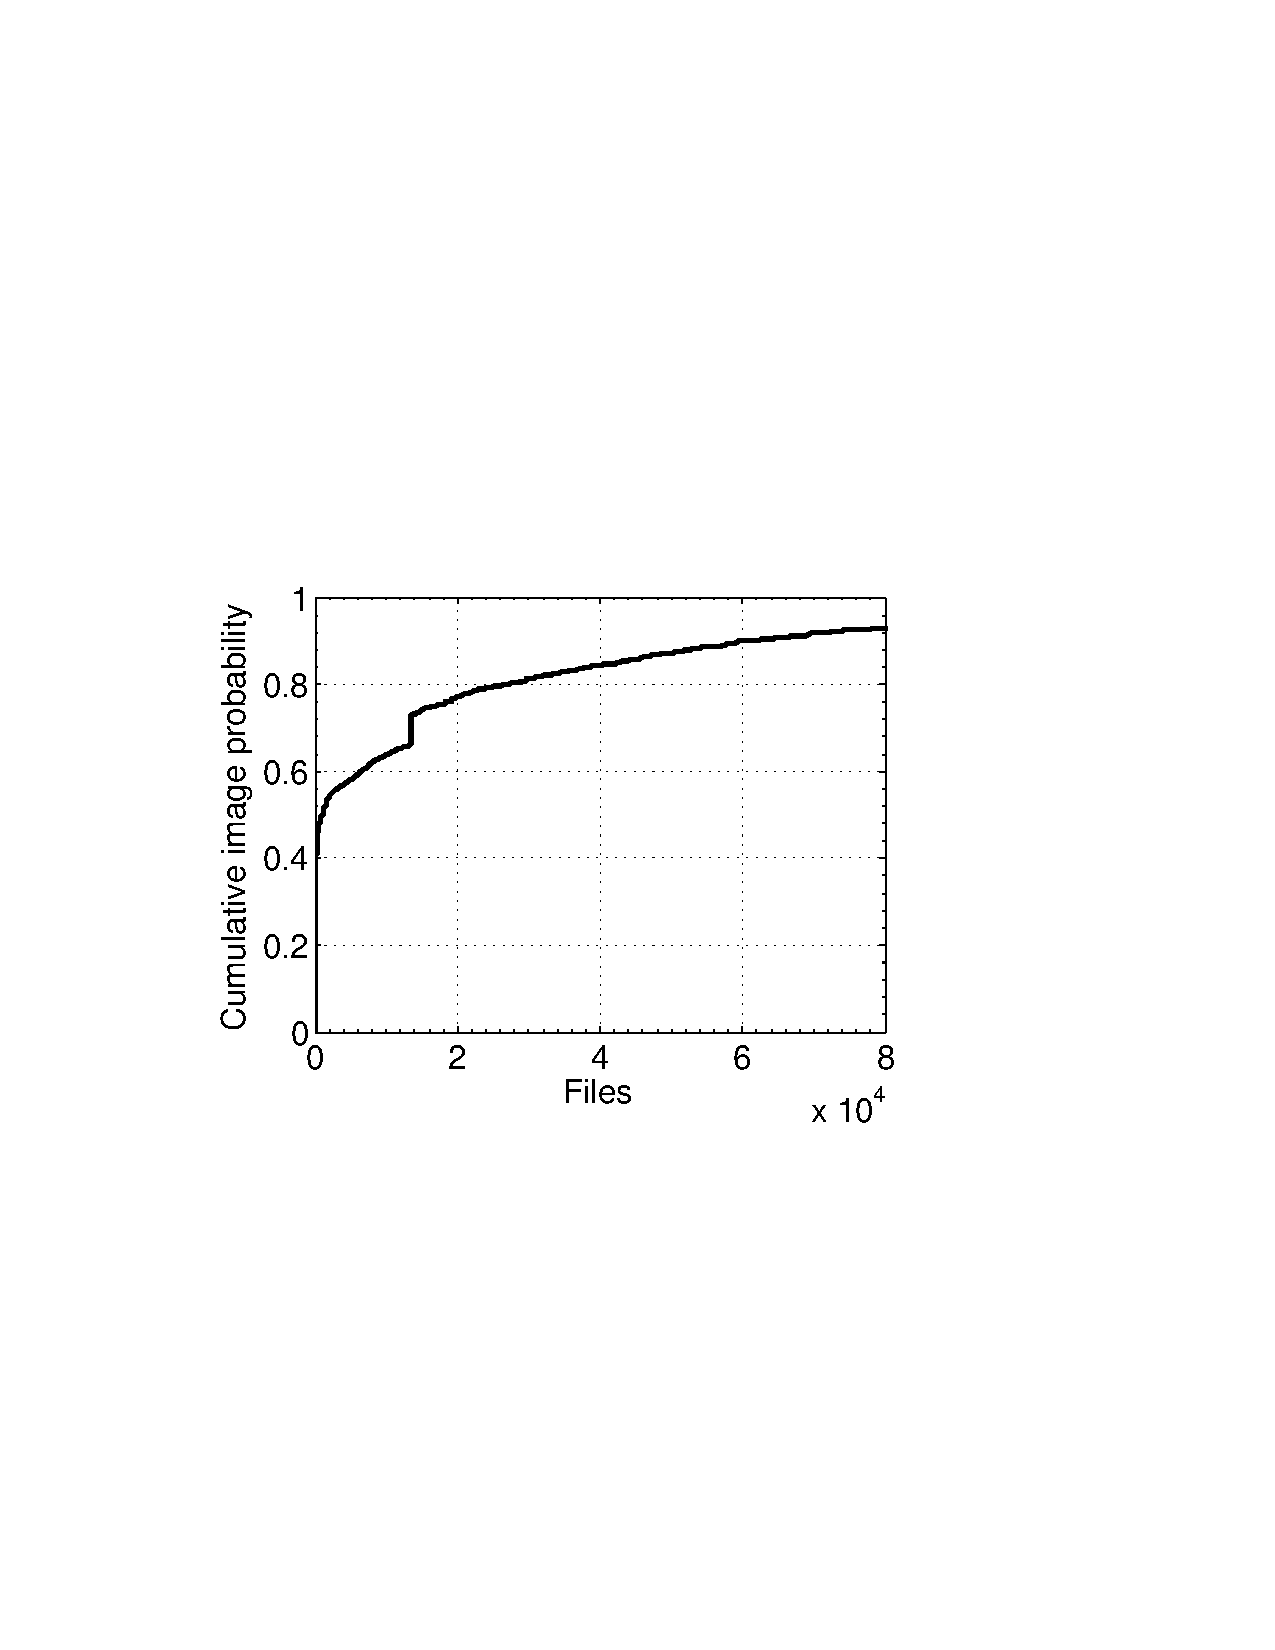
\includegraphics[width=1\textwidth]{graphs/file.pdf}
%		\caption{CDF of images by files}
%		\label{fig-file}
%	\end{minipage}
%\end{figure}

%\begin{figure}[htbp] 
%	\begin{minipage}{0.5\linewidth} 
%		\centering 
%		\includegraphics{circle} 
%		\caption{A Circle} 
%		\label{fig:circle} 
%	\end{minipage}% 
%	\begin{minipage}{0.5\linewidth} 
%		\centering 
%		\includegraphics{rectangle} 
%		\caption{A Rectangle} 
%		\label{fig:rectangle} 
%	\end{minipage} 
%\end{figure}

%\begin{figure}[t]
	\centering
%		\begin{minipage}{0.23\textwidth}
%			\centering
%			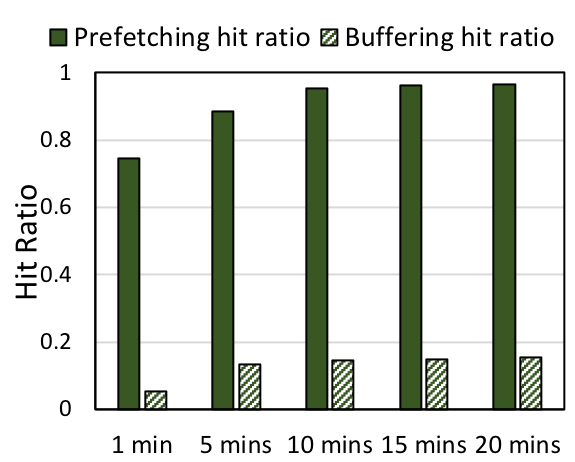
\includegraphics[width=1\textwidth]{graphs/evaluation_hitratios.png}
%			\caption{Hit ratio.}
%			\label{fig:hitratio}
%		\end{minipage}
	%	\begin{minipage}{0.25\textwidth}
			\centering
			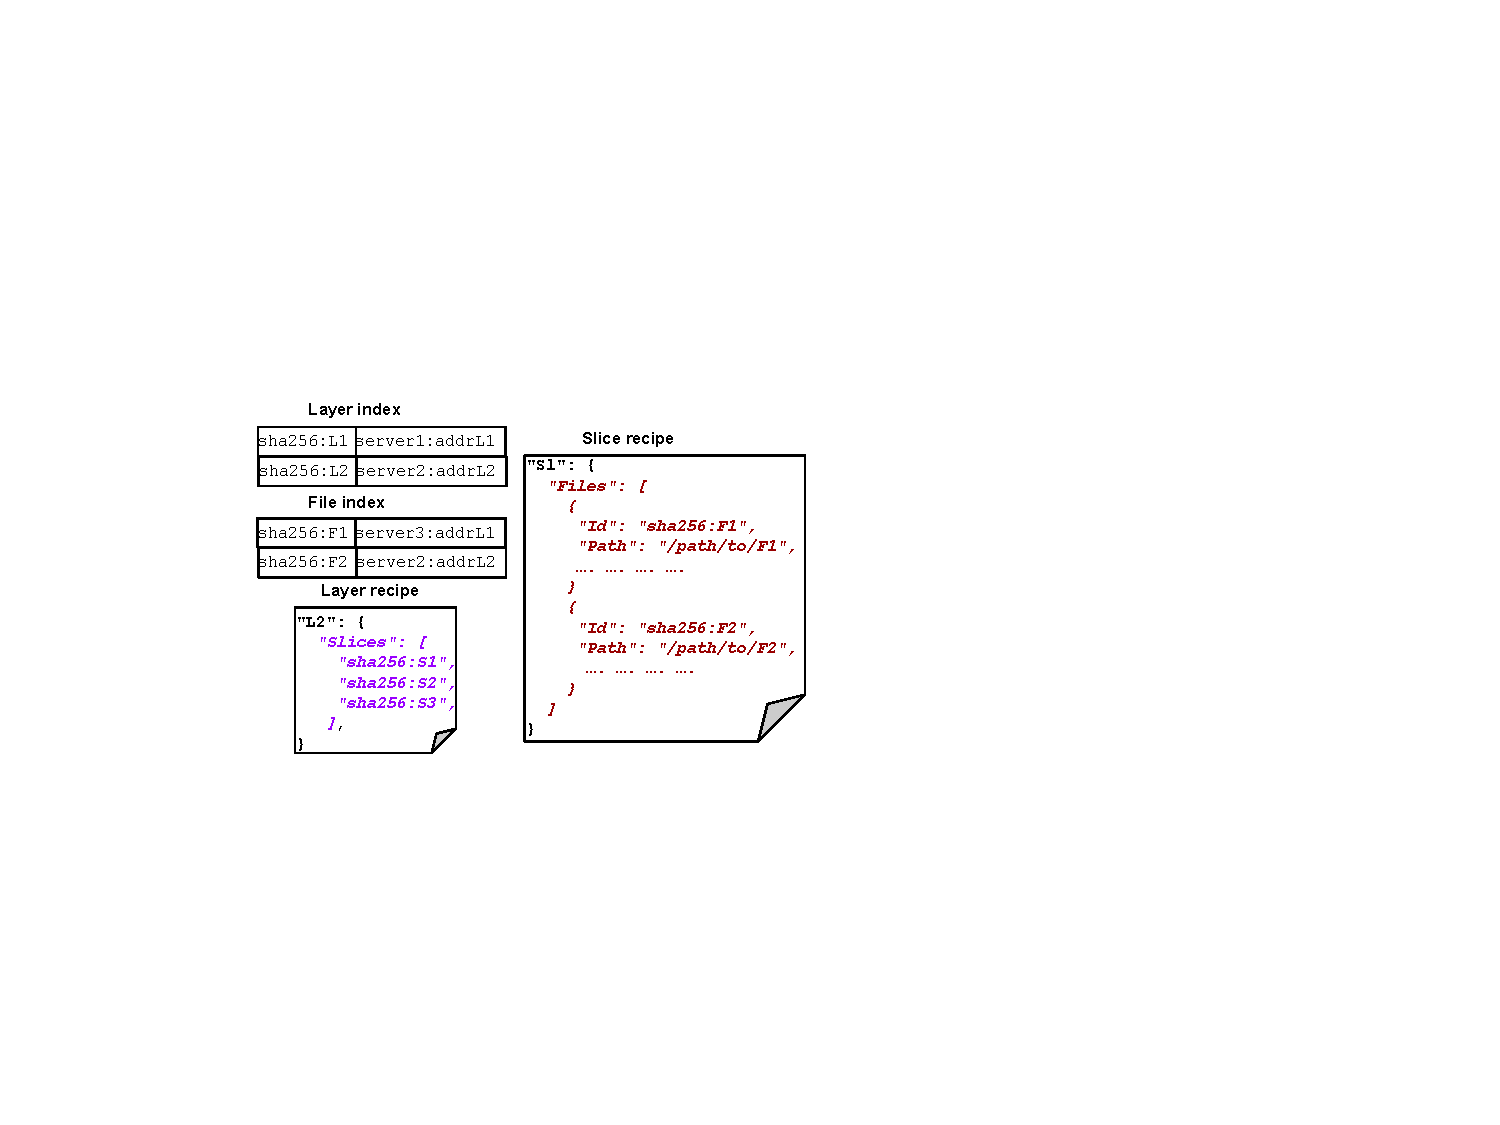
\includegraphics[width=0.4\textwidth]{graphs/sift-metadata.pdf}
			\caption{Metadata for deduplication.}
			%\vspace{-3pt}
			\label{fig:sift-metadata}
	%	\end{minipage}
\end{figure}
\paragraph{Layer file-level deduplication}
As shown in Figure~\ref{fig:dedup-partition}, 
a layer is loaded to layer deduplication process.
First, the layer is decompressed and unpacked into files.
Next, 
the process computes a \emph{fingerprint} for every file denoted as \textbf{file id}, 
and checks every file's fingerprint in the file index.
If the file is already stored, it will be discard. 
Otherwise, it will be kept in file store.
Meanwhile,
\sysname  records the newly added \emph{file id} to file index.
\paragraph{Layer partition}
%Note that, layer deduplication process only deduplicates regular files., 
After removing file duplicates,
deduplication process distributes the layer's remaining files to different registry servers
so that each server is able to rebuild an $\sim$equal-sized slices for the layer from its local file store.
Then, the process sends slices to the corresponding registries.
Finally, \sysname will add slice recipes and layer recipe to metadata database as shown in Figure~\ref{fig:dedup-partition}.

\begin{algorithm}
\scriptsize 
	\caption{Layer deduplication and partitioning}
	\label{alg:dedup-partition}
	\KwIn{\\	
			$FileIndex$: File index. \\
	}

	\KwOut{\\
			$LayerRecipe$: Layer recipe for layer $L$.\\
			$SliceRecipes$: Slice recipes for layer $L$' slices.\\
	}

	archive $\leftarrow$ \texttt{Decompress} layer $L$ \\

	\ForEach{header, content in archive} 
	{ 
		Id $\leftarrow$ \texttt{Hash} content \\
		%destHeader $\leftarrow$ header \\
		\eIf{ Id in FileIndex}{
			host  $\leftarrow$ $FileIndex$[Id].host \\
			src $\leftarrow$ $FileIndex$[Id].header \\
			{\tiny\texttt{/* SliceRecipe is identified by `layerid::host'}}
			SliceRecipe[$L::host$] $\leftarrow$  \texttt{Add} (header, src) \\
			{\tiny\texttt{/* Skip redundant file.  }}\\
		}{
			{\tiny\texttt{/* create file with content in file store.  }}\\
			file $\leftarrow$ \texttt{Create and write} content \\
			src $\leftarrow$ \texttt{Stat} file \\
			entries $\leftarrow$ (header, src)  \\
		}
	}
	
	\Do{entries}{
		{\tiny\texttt{/* get file entry with maximum file size. }}\\
		maxFile $\leftarrow$ \texttt{Max} entries \\
		{\tiny\texttt{/* get smallest slice. }}\\
		minSlice $\leftarrow$ \texttt{Min} SliceRecipes \\
		{\tiny\texttt{/* assign biggest file to smallest slice. }}\\
		minSlice $\leftarrow$ \texttt{Add} maxFile \\
		{\tiny\texttt{/* Set maxFile to FileIndex}}\\
		{\tiny\texttt{/* Remove maxFile from entries. }}\\
	}
	{\tiny\texttt{/* Send slices.}}\\
	{\tiny\texttt{/* Set SliceRecipes.}}\\
	{\tiny\texttt{/* Include all slices' hosts to workers.}}\\
	{\tiny\texttt{/* Select biggest slice' host as master.}}\\
	{\tiny\texttt{/* Set LayerRecipe.}}\\
	
	
		
\end{algorithm}




Algorithm~\ref{alg:dedup-partition} details layer deduplication and partition.
After decompression, 
each file entry in the layer archive is represented as a \textbf{file header} and \textbf{file content}.
File header contains file name, path, size, mode, owner information, etc.
Note that file header is needed to rebuild the \emph{file header} for 
associated file entry in the layer archive.

%During layer deduplication process,
\sysname records each file entry's file header and 
calculates the file id by hashing the file content.
As mentioned, file index maps a \emph{file id} to its associated physical file stored in file store.
To address a physical file,
each file id in the file index holds its 
%denoted by a combination of its 
\emph{host address} and \textbf{file status} of the physical file which mainly contains file name, path, and size.
As shown in Algorithm~\ref{alg:dedup-partition}, 
if a file's file id already exists in file index, 
this file will be added to its host's corresponding partition (i.e, slice). 
Otherwise,
\sysname stores file content as a physical file in file store
and retrieves the file status of the physical file.
File index is updated accordingly.

Slice recipe is identified by a simple combination of layer id and its host registry address,
denoted as $layerid::host$ as shown in Algorithm~\ref{alg:dedup-partition}.
Slice recipe represents a layer partition and
is used to construct a partial layer,
which
records each file entry' $header$ in the layer archive partition and 
its corresponding physical file's status $src$. 
In this case, 
each file is represent as a $header$ in the layer archive and
its corresponding physical file's status $src$. 


%After unpacking the layer archive, 

%Note that destHeader can be used to rebuild the \textbf{file header} for 
%associated file entry in the layer archive.

 %its host' slice
%to get identical files' server addresses.
To distribute the newly added unique files,
\sysname uses a greedy partition algorithm to 
assign the biggest file to the smallest slices
such that layer can be evenly partitioned among registry servers.
%After layer partition,.
All the slices' hosts are denoted as layer restoring \textbf{workers}. 
Next, \sysname stores slice recipes in metadata database after successfully
sending slices to their corresponding workers.
\sysname selects the biggest slice' host as layer restoring \textbf{master}.
Layer recipe records the workers and master information for layer restoring.
Finally, \sysname stores layer recipe in metadata database.
%Layer recipe 

%Here, we use the metadata database as a distributed lock for file index.
%File index sets a file id to hold  only if the file id does not exists.

%it uses a weighted round robin algorithm to distribute newly added 
%unique files to the registry cluster. These servers that already contains this layer's identical files
%are assigned a lower weight. 
%This is to ensue that different servers maintain same amount of files that are needed to restoring equal sized 
%slices for this layer.
%Deduplication process also 
%updates the \emph{file index} with the newly added unique files' fingerprints and host addresses.   
%Then, it calculates the slice fingerprints and creates a slice recipe for each slice.
%Slice recipe contains partial of the layer tarball's directory tree structure, file fingerprints, file name along with file path in the tarball, and file metadata information 
%(such as permissions and creation date), which are needed for restoring a slice for the layer. 

%After that
%After removing the duplicate files,
%Then, it
%distributes the \emph{deduplicated slices} evenly to the registry cluster by using round-robin, and,
%In the end, deduplication process creates a layer recipe which contains its slices' fingerprints and 
%based on layer recipe, it updates image manifests.
%The layer's tarball and file duplicates are removed after deduplication.

\subsection{Layer restoring}

%\paragraph{Parallel slice restoring}
%\label{subsubsec:slice-restoring}



\begin{figure}[t]
	\centering
	\centering
	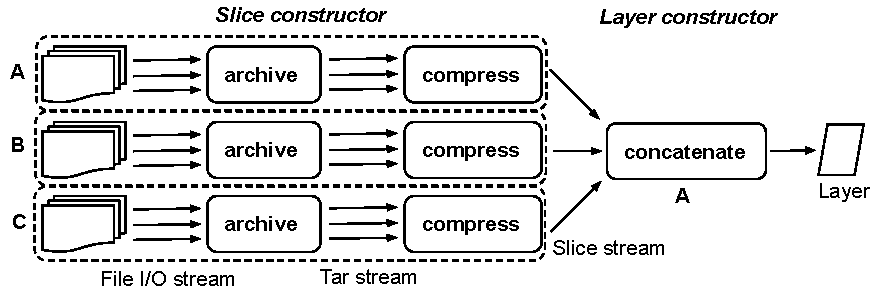
\includegraphics[width=\columnwidth]{graphs/sift-layer-construct-new.pdf}
	\caption{Parallel streaming layer construction.}
	\label{fig:construct}
\end{figure}



When a~\texttt{pull} layer request is received, 
\sysname will first search layer diskcache.
If not found,
\sysname will rebuild the layer from file store according to its layer recipe. 
%the \dedupname~system 
%first prepares a directory structure for the slice, based on the slice recipe.
%Then, it copies the files into the directory tree.
%Next, it compresses the slice's directory tree into a slice tarball,
%and directly sends it back to the client.

\paragraph{Parallel layer construction}

When a~\texttt{pull} layer request is received, 
\sysname will update \emph{ULmap}. 
ULmap records user access status,
which maps a \textbf{user id} to its accessed layers with its corresponding access count,
where user id is defined as client request address.

Upon a \texttt{pull} layer request miss, 
\sysname initiates a layer restoring process for it.
The process has two parts: slice constructor and layer constructor.
Figure~\ref{fig:restoring} shows an example of parallel layer restoring when a \texttt{pull} layer request miss happens.
First, 
layer constructor fetches the layer recipe from metadata database.
As shown in $L1$'s layer recipe, 
the restoring workers contains registry $A$, $B$, and $C$.
Since registry $A$ is the restoring master,
it sends ``\texttt{Get slice}" requests to its peer workers: $B$ and $C$.
After a \texttt{Get slice} request is received, 
$B$ and $C$ start slice construction and return a slice back to $A$ respectively.
Meanwhile $A$ instructs local slice constructor to rebuild a slice for $L1$.
Slice constructor first gets its associate slice recipe from metadata database 
keyed by a combination of  layer id and registry address (``$L1::A$").
Then, based on slice recipe,
slice constructor fetches files pointed by $Srcs$
and builds a slice archive.
After receiving all slices, layer constructor concatenates them into a compressed layer
and sends back the client. 

\paragraph{Streaming layer construction}
Figure~\ref{fig:construct} details the stateless streaming layer construction process.
First, slice constructor loads file in parallel from file store based on the slice recipe.
Each file is written to an archive buffer asynchronously.
Before writing file content to the archive buffer, slice constructor first builds and writes its
associated 
file header into the archive buffer according to the slice recipe. 
After archiving all the files in the slice,
the archive buffer will be divide into few chunks and compressed in parallel,
then concatenated into a single compressed slice stream.
Through network transfer, multiple slice streams will be concatenated into a single layer.
No intermediate file will be created or stored on disk.

\sysname uses a small file cache to reduce file I/Os. 
File cache uses LFRU replacement policy.

%headers according to $Dests$,
%after that it writes file contents into the archive
 
%Slice restoring process has four suboperations: 
%slice recipe lookup,
%slice file copying,
%slice compression, and
%slice network transfer. 
%To measure the overhead for each suboperation, 
%we implemented layer deduplication and parallel slice
%restoring on a 4-node registry cluster. 
%We first warmup the cluster by pushing 200 layers to the cluster
%and initiating layer deduplication process.
%The layers were randomly selected from our layer dataset detailed in xxx limited to 50MB.
%After finishing layer deduplication,
%we sent 400 \texttt{pull slice} requests to the cluster with 10 \texttt{pull slice} requests issued at a time.
%Figure~\ref{fig:slice-restoring-breakdown} shows the CDFs of the latencies for each suboperation.
%We see that across the four suboperations,
%the duration for slice compress is the shortest.
%Slice compression only took less than 0.001 s because a slice is a smaller unit. 
%The next shortest suboperation is network transfer since we pulled layer slice through Ethernet.
%90\% of slice recipe lookups took less than 0.1 s while 
%the highest slice recipe lookup duration almost reaches 0.8 s,
%which is caused by high concurrent lookup requests 
%%(note that we use redis to store metadata \NZ{use mongodb instead}).
%The most time consuming suboperation is slice file copying, which involves 
%copying all 
%the files that belong to the slice to their destination directory based on the slice recipe.
%Note that we implemented a thread pool on each registry server to read files in parallel
%and write data in RAMdisk to reduce disk IOs.
%40\%of slice file copying duration is greater than 1 s and 
%10\% of slice file copying duration is higher than 10 s.
%This is because bigger slices contains more files and requires more disk IOs.
%The overhead of slice copying can be largely mitigated for a large-scale registry cluster
%since the size of slice roughly equals to $S_{l}/N$, where $S_{l}$ denotes the layer size and $N$ is size of registry cluster.
%However, it could be a bottleneck for slice restoring on a small-scale registry cluster.
%%and slice file copying duration depends on slice size.
%
%%\begin{algorithm}
\scriptsize 
	\caption{File cache assisted slice restoring}
	\label{alg:file-cache}
	\KwIn{\\
		$\theta_{rsfc}$: Slice restoring latency threshold. \\
		$s$: Slice to be restored. \\
	}

	\SetKwFunction{Fsub}{Restore}
	\SetKwProg{Fn}{Function}{:}{}

	\Fn{\Fsub{s}}{
		%{\tiny\texttt{/* Otherwise, it's a repull layer miss   /}}\\
		\eIf{files in s are cached in file cache}
		{
			slice $\gets$ \texttt{RestoreSlice} \emph{s} \texttt{From} \emph{file cache + disk} 
		}
		{
			slice, $D_{rs}$ $\gets$ \texttt{RestoreSlice} \emph{s} \texttt{From} \emph{disk} \\
			\If{ $D_{rs} > \theta_{rsfc}$} 
			{ 
				\emph{file cache} $\gets$ \texttt{Cache} \texttt{Subsetof} \emph{s.files}
			}		
		}
	}

\end{algorithm}



%
%To reduce slice file copying overhead,
%\sysname~\filecachename~temporally cache a subset of unique files for bigger and popular slices that have a high slice restoring latency, ie., $D_{rs} > \theta_{rsfc}$, 
%where $D_{rs}$ is the slice restoring latency and $\theta_{rsfc}$ is the restoring latency threshold for 
%caching
%a subset of files from the slice to help improve its restoring performance as shown in Algorithm~\ref{alg:file-cache}.
%Upon a \texttt{pull slice} request for those slices, 
%\dedupname~ system fetches a subset of its containing files from \filecachename~and
%the remaining files from disk for slice restoring.
%
%To identify which slices have a high slice restoring latency,
%\dedupname~system monitors slice restoring performance and 
%maintains a restoring performance  profile for each slice that has been restored,
%% as shown in Figure~\ref{fig:xxx},
%which contains the latency breakdown of slice restoring
%% (,and a decompression latency updated by layer decompression process) 
%and its containing files' sizes.
%All the slice restoring performance profiles are also stored in distributed  databases,
% and addressed by slice digests. 
%To estimate the restoring latency for a slice $i$ that hasn't been restored, 
%\dedupname system~first lookups the slice restoring performance profiles by slice size,
% then selects a slice $x$ that is most similar in size to $i$,
% and estimates $i$'s restoring latency as: 
% $D_{rs}(i) \approx D_{rs}(x) + \Phi_{rs}(\Delta_{S})$,
% where $\Delta_{S}$ is the size different between two slices.
% $\Phi_{rs}(\Delta_{S})$ denotes a slice restoring latency function of slice size variation.
%  $\Phi_{rs}(\Delta_{S})$ is generated by using linear regression~\cite{xxx}.
% %$\varepsilon_{rs}$ is the standard error of restoring latency estimation for the layers similar in size.
%If the estimated slice restoring $D_{rs}(i) > \theta_{rs}$,
%then, \dedupname~lookups the slice restoring performance profiles by slice size,
%selects a slice $y$ that has a acceptable restoring latency and
%most similar in size to $i$.
%Next, \dedupname system~caches a subset of files $F$ for slice $i$, so that
%$D_{rs}(i) - \Phi_{rs}(\Sigma_{S}(F)) \approx D_{rs}(y)$,
%where $\Sigma_{S}(F)$ is the sum size of files in $F$.
%
%Note that \filecachename~size is limited so that \filecachename~only caches 
%subsets of files for big slices that belongs to popular layers.
%%that will be accessed later. 
%\cref{sec:cache-design} will describe how to determine popular layers based on user access patterns.
%Note that the slices for the same layer have similar sizes, restoring latencies, and popularity 
%because of unique file
%distribution. 
%Thus, once a layer is determined as popular layer, 
%\dedupname~will cache similar amount of files for its slices.
%Note that all the files in file cache are unique and can be shared for restoring different slices.
%
%For on-premise or private registry cluster, the network transfer speed is usually faster than remote cloud.
%Thus, slice compression is less important for medium to small size slices, 
%especially for the slices that have a high decompression latency, 
%i.e., $D_{stt} < \theta_{stt}$ and $D_{dc} > \theta_{dc}$, where $D_{stt}$ and $D_{dc}$ denote slice transfer duration
%and decompression duration respectively; 
%$\theta_{stt}$ and $\theta_{dc}$ denote thresholds for them respectively.
%Consequently, \dedupname system~only archives these slices without compressing them and directly sends
%these archival files back to the clients to eliminate clients' decompression latency.



